% ===========================================================================================================
% TEX file generated by R with the 'knitr' package
%
% DO NOT EDIT THE TEX FILE DIRECTLY
% ===========================================================================================================

\documentclass[a4paper,PageStyleII,12pt,times,numbered,print]{Class/PhDThesisPSnPDF}\usepackage{knitr}

% Captions in floating environments
\usepackage[labelsep=colon,tableposition=top,font=small,margin=5pt,format=hang]{caption}

% For subcaptions in figures
\usepackage{subcaption}

% For sidewaysfigure
%\usepackage{rotfloat}

% For professional looking tables
\usepackage{booktabs} 

%\usepackage{multirow}
%\usepackage{multicol}
%\usepackage{longtable}
%\usepackage{tabularx}

% For underscores that correspond to the encoding
\usepackage[T1]{fontenc}

% For \FloatBarrier
\usepackage[section,below]{placeins}

% Linebreaks in tables
\usepackage{makecell}

% Hyperlinks
\usepackage{hyperref}

% Table of content settings
\setcounter{tocdepth}{2}
\setcounter{secnumdepth}{2}

% Allowed percentages of page a float can use
\renewcommand{\textfraction}{0.05}
\renewcommand{\topfraction}{0.95}
\renewcommand{\bottomfraction}{0.95}
\renewcommand{\floatpagefraction}{0.75}
\setcounter{totalnumber}{5}

% Figure names
\renewcommand{\figurename}{Fig.}

% changes the default name `Bibliography` -> `References'
\renewcommand{\bibname}{References}

\newenvironment{romanpages}{
  \setcounter{page}{1}
  \renewcommand{\thepage}{\roman{page}}}
{\newpage\renewcommand{\thepage}{\arabic{page}}}

% Used for knitr images from Rnw files
\newcommand{\subfloat}[2][default for first parameter: need a sub-caption]{\subcaptionbox{#1}{#2}}

% Typesetting commands
\newcommand{\R}{\textbf{\textsf{R}}}


% ************************ Thesis Information & Meta-data **********************
%% The title of the thesis
\title{Thesis Template using R and knitr}
%\title{Writing your PhD thesis in \texorpdfstring{\\ \LaTeX2e}{LaTeX2e}}
%\texorpdfstring is used for PDF metadata. Usage:
%\texorpdfstring{LaTeX_Version}{PDF Version (non-latex)} eg.,
%\texorpdfstring{$sigma$}{sigma}

%% Subtitle (Optional)
%\subtitle{Using the CUED template}

% Crest minimum should be 30mm.
%\crest{\includegraphics[width=0.25\textwidth]{THK}}

%% The full name of the author
\author{Alexis Marino Sard\'a Espinosa}

%% University and Crest
\university{DBZ}

%% Department (eg. Department of Engineering, Maths, Physics)
\dept{Faculty of Computer Science and Engineering}

%% College shield [optional] 
% Crest minimum should be 30mm.
%\collegeshield{\includegraphics[width=0.2\textwidth]{CollegeShields/Kings}}

%%% This is the default option, the hack I did with College affiliation looks better in my opinion...
%%% and apparently right now it only works with one supervisor by default...

%% Supervisor (optional)
%\supervisor{Prof. Dr. Thomas Bartz-Beielstein}
% Supervisor Role (optional) - Supervisor (default) or advisor
%\supervisorrole{First Examiner: }

%% Supervisor (optional)
%\supervisorSecond{Dr. Ing. Subanatarajan Subbiah}
% Supervisor Role (optional) - Supervisor (default) or advisor
%\supervisorrole{Second Examiner: }

%% You can redefine the submission text:
% Default as per the University guidelines:
% ``This dissertation is submitted for the degree of''
%\renewcommand{\submissiontext}{change the default text here if needed}

%% Full title of the Degree
\degreetitle{Master of the Universe}

%% Submission date
% Default is set as {\monthname[\the\month]\space\the\year}
%\degreedate{\monthname[\the\month] \\ \the\year} 

\IfFileExists{upquote.sty}{\usepackage{upquote}}{}
\begin{document}



% ===========================================================================================================
% Cover
% ===========================================================================================================

\frontmatter

\begin{titlepage}
  \maketitle
\end{titlepage}

% ===========================================================================================================
% Front matter
% ===========================================================================================================

\pagenumbering{Roman}

\begin{dedication}
To me
\end{dedication}

\begin{abstract}
Abstract goes here
\end{abstract}

\begin{declaration}
I declare that..
\end{declaration}

\begin{acknowledgements}
I want to thank...
\end{acknowledgements}

\tableofcontents

\listoffigures

\listoftables

%\printnomenclature

% ===========================================================================================================
% Main matter
% ===========================================================================================================

\mainmatter

\chapter{Introduction}
\label{ch:introduction}

\section{Introduction}
\label{sec:introduction}

I did my thesis in \R{}, and it took me a while to get everything working the way I wanted. The example here is a skeleton that could serve as a starting point to write not only theses, but any kind of document using \LaTeX{} and \R{}.

The main files have a \texttt{Rnw} extension and are transformed into \texttt{tex} files by using the \texttt{knitr} package.\footnote{\url{http://yihui.name/knitr/}} However, anything that doesn't depend on \R{} can be written directly in \texttt{tex} files, making it flexible.

I didn't put too much effort into the layout shown here, it is only meant to serve as a starting point with some examples. Other templates can also be used.


\chapter{Organization}
\label{ch:organization}

\section{Compilation Scripts}
\label{sec:comp-scripts}

There are two main files used for compilation: \texttt{compile-linux} for Linux users, and \texttt{compile-windows.bat} for Windows users. They are both used in the same manner, so in the examples below I will simply refer to the scripts as \texttt{compile}.

The first thing that is needed is of course \LaTeX{}. There are many resources available on how to install it, so I will not dwell on that.

The next thing is \R{} itself. Again I will not go into too much detail, just make sure that the \texttt{Rscript} executable is available in your path. If you have code that will use parallel computation, the default \R{} package that is used is \texttt{doParallel}, although this can be modified in the file \texttt{Thesis.R} (see Section~\ref{sec:main-files}).

If you simply double click on the \texttt{compile} script, it will run \texttt{pdflatex}, \texttt{bibtex} and \texttt{pdflatex} twice (for citations to work). This will apply any changes made to any \texttt{tex} file, but will \textbf{not} detect any changes made in \texttt{Rnw} files, regardless of whether it's \R{} code or not. Running the scripts from the command line with no arguments is equivalent.

The other option is to run the scripts from the command line followed by a single argument, either \texttt{TRUE} or \texttt{FALSE}; this will \textit{knit} the main \texttt{Thesis.Rnw} file and apply all changes made, including \R{} code. If you use \texttt{FALSE}, everything is done sequentially. With \texttt{TRUE}, a number of parallel workers equal to the number of detected CPU cores are registered first, so that \R{} code can run in parallel. This is only useful if your code is specifically made to run in parallel (e.g. with the \texttt{foreach} package).

\section{Main Files}
\label{sec:main-files}

If the \texttt{compile} scripts are called to update the \R{} code, they basically call \texttt{Rscript} on \texttt{Thesis.R}. The latter registers the parallel workers if necessary and calls \texttt{knitr} on \texttt{Thesis.Rnw}, which creates \texttt{Thesis.tex}. It also loads \R{} utilities on each worker (see Section~\ref{sec:utilities}).

The master file is \texttt{Thesis.Rnw}, which contains the main \texttt{tex} layout as well as the defaults for \texttt{knitr} (more on that in Section~\ref{sec:default-func}).

\subsection{Utilities}
\label{sec:utilities}

By ``utilities'' I mean the common \R{} functions and libraries that will be used. I have made a basic distinction between cached and uncached utilities. This is related to \texttt{knitr}'s cache function, so you should definitely read about that first if you don't know how it works. Uncached utilities should be the ones that will be used by \texttt{knitr} itself or in the chunk options.

The files are located in the \texttt{Utils} folder and have obvious names\dots

\section{Default Functionality}
\label{sec:default-func}

\subsection{Knitr Cache}

You can see the defaults for \texttt{knitr} in \texttt{Thesis.Rnw}. By default, all chunks are cached and hidden from the output (with \texttt{echo = FALSE}). Additionally, auto-dependency detection is turned on by default; this has worked well for me.

Uncached utilities are always loaded along with \texttt{knitr}'s defaults. The rest of the used libraries and functions can be included in the cached utilities file.

Cache is created in \texttt{Data/cache/}.

\subsection{MD5 Hashes}

I've included a function called \texttt{md5} that I've used in some chunk options. Since you can add any non-NULL value to chunk options in order to create its cache (again, read \texttt{knitr}'s information on cache if you haven't), you can use MD5 hashes to create chunks that depend on specific files, so that if the files change, the chunk will be updated automatically. There is an example of this in the source code for Section~\ref{sec:basics}.

It is a semi-custom function because the default \texttt{md5sum} doesn't throw an error if it doesn't find the file, in which case you might not notice if you're actually caching a valid file or not.

\subsection{Workspace Cleaning}

I also include a function called \texttt{clean\_workspace} that removes everything except the uncached utilities. It can optionally reload cached utilities and ignore variables if desired. 

I run this at the end of each child \texttt{Rnw} file. I do this because I'm not sure how \texttt{knitr}'s auto-dependency detection works (my bad), and I wanted each child file to be as independent as possible so that things wouldn't break in one section if I changed something from the previous section. Check the source code for the examples, and note that this cleaning is always uncached.

\subsection{Dynamic Loading of Utilities}

I was using several libraries, and it was annoying to wait for all of them to load if all I wanted to do was update content without changing any \R{} code (recall that changes made to \texttt{Rnw} files won't be detected unless you re-knit everything). My solution was to use a \texttt{knitr} hook (see \texttt{knitr}'s website).

The hook is a function called \texttt{utils\_hook}, located in the uncached utilities file. If you see the defaults in \texttt{Thesis.Rnw}, you'll notice every chunk will run the hook by default, which loads cached utilities before actually running the chunk. Since the hooks are only executed if the chunk needs to be updated (i.e. its cache was invalidated or non-existent), utilities are only loaded whenever I actually have to re-run \R{} code. Each chunk that needs to be updated will re-load everything, of course, but that's unimportant (i.e., re-loading a library has no effect).

Notice that chunks that are manually uncached should set the \texttt{load.utils} hook option to NULL to avoid loading things unnecessarily. See the source code for workspace cleaning chunks for examples.

\subsection{Tables}

I used the \texttt{xtable} package to create tables from data frames. I created a (cached) function called \texttt{make\_table} that has some defaults so that I didn't need to write everything every time. You can see the defaults in the source code and note that any default can be overridden via the ellipsis.

The \texttt{results} chunk option should be set to \texttt{"asis"} so that everything is detected correctly. See the source code for Section~\ref{sec:tables}.

\subsection{Random Seeds}

I set one overall seed in the initial chunk where \Texttt{knitr} is configured. I've added another hook (\texttt{seeds\_hook}) that saves the random seed for every chunk (by default) and restores it whenever it is run, in order to maintain reproducibility. The seeds are saved in the \texttt{Data/seeds.RData} file. It should detect new chunks, and the chunk labels are used for naming. If you want to disable this for a given chunk, add \texttt{rand.seed = NULL} to the chunk options (see, e.g., the last chunks in the files in the \texttt{Examples} folder).

Note that when adding/modifying chunks after initial caching, it could be that some or all chunks end up with new random seeds, especially if some chunks are not cached. If there is a chunk whose reproducibility is crucial, set its seed manually inside the chunk. Alternatively, manually open the seeds file, delete the seeds you want to update, and manually save it again.

\section{Considerations}
\label{sec:considerations}

\subsection{File Paths}

Be careful with paths, for example you should specify the correct figure path in both \texttt{knitr} and \LaTeX{} options; see the source code for Section~\ref{sec:figures}.

Additionally, you should know that each child \texttt{Rnw} file is run with its own directory as the working directory. However, the paths you give to \texttt{knitr} or the ones used in chunk options are always with respect to the root directory, i.e. where \texttt{Thesis.Rnw} is located. See the source code for Section~\ref{sec:basics} for an example.

\subsection{Chunk Names}

I believe all chunk names need to be unique.


\chapter{Examples}
\label{ch:examples}


\section{Basics}
\label{sec:basics}

The \texttt{caret} package is one that can take advantage of parallel execution. Below, I train a random forest on a sample dataset~\cite{lichman2013}.

% This chunk depends on the MD5 of chess.txt; if that file changes, the chunk needs to be updated


\begin{knitrout}
\definecolor{shadecolor}{rgb}{0.969, 0.969, 0.969}\color{fgcolor}\begin{kframe}
\begin{alltt}
\hlkwd{set.seed}\hlstd{(}\hlnum{3830}\hlstd{)}

\hlstd{chess_rf} \hlkwb{<-} \hlkwd{train}\hlstd{(label} \hlopt{~} \hlstd{.,} \hlkwc{data} \hlstd{= chess,}
                  \hlkwc{method} \hlstd{=} \hlstr{"rf"}\hlstd{,}
                  \hlkwc{tuneGrid} \hlstd{=} \hlkwd{data.frame}\hlstd{(}\hlkwc{mtry} \hlstd{=} \hlnum{8}\hlopt{:}\hlnum{15}\hlstd{),}
                  \hlkwc{trControl} \hlstd{=} \hlkwd{trainControl}\hlstd{(}\hlkwc{method} \hlstd{=} \hlstr{"oob"}\hlstd{))}

\hlstd{best} \hlkwb{<-} \hlstd{chess_rf}\hlopt{$}\hlstd{bestTune}\hlopt{$}\hlstd{mtry}
\hlstd{acc} \hlkwb{<-} \hlkwd{round}\hlstd{(chess_rf}\hlopt{$}\hlstd{results}\hlopt{$}\hlstd{Accuracy[chess_rf}\hlopt{$}\hlstd{results}\hlopt{$}\hlstd{mtry} \hlopt{==} \hlstd{best],}
             \hlnum{3}\hlstd{)}
\end{alltt}
\end{kframe}
\end{knitrout}

Using a random forest with the Chess dataset and OOB error estimate, best value of \texttt{mtry} was 13 with an accuracy of 0.995.

Try changing the seed (to invalidate the chunk's cache) and compiling the thesis with/without parallel support to see the difference in run time.

If you don't specify a seed, you might lose reproducibility. For example, the code below might give a different result each time you recompile if you add code before it and \textit{after} the cache for the previous chunk has been created. This is because the previous chunk will no longer set the seed unless its cache is invalidated and the chunk is thus updated.

\begin{knitrout}
\definecolor{shadecolor}{rgb}{0.969, 0.969, 0.969}\color{fgcolor}\begin{kframe}
\begin{alltt}
\hlkwd{rnorm}\hlstd{(}\hlnum{1}\hlstd{)}
\end{alltt}
\begin{verbatim}
## [1] 0.1699193
\end{verbatim}
\end{kframe}
\end{knitrout}




\section{Figures}
\label{sec:figures}



\graphicspath{Examples/Figs/}

Plots can be created directly in \R{} and the results are added automatically to the \texttt{tex} file. See Fig.~\ref{fig:iris-histograms} for an example of a single plot.

\begin{knitrout}
\definecolor{shadecolor}{rgb}{0.969, 0.969, 0.969}\color{fgcolor}\begin{figure}[htpb]

{\centering 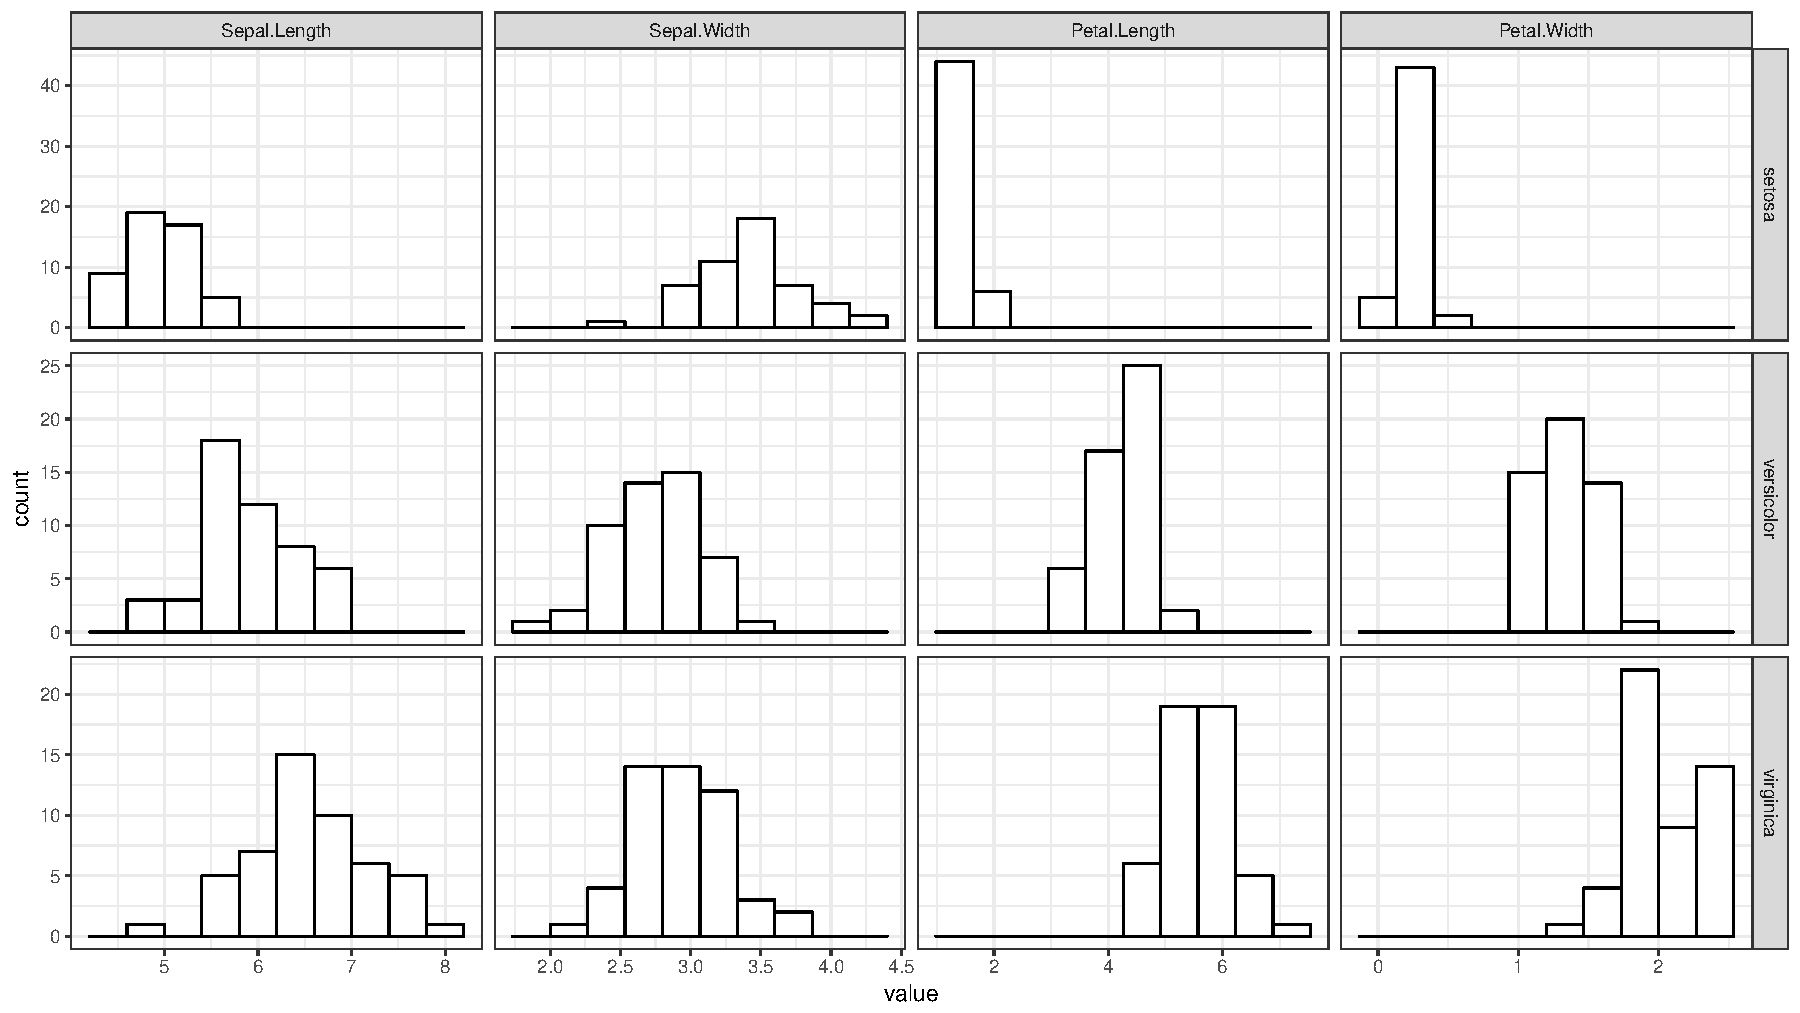
\includegraphics[width=\linewidth]{Examples/Figs/iris-histograms-1} 

}

\caption[Histograms for the iris dataset]{Histograms for the iris dataset. Look at the list of figures to see difference between short and long captions.}\label{fig:iris-histograms}
\end{figure}


\end{knitrout}

You can create several plots per chunk and have them in the same main figure. See Fig.~\ref{fig:mtcars-subplots} for an example of two plots: Fig.~\ref{fig:mtcars-subplots1} and Fig.~\ref{fig:mtcars-subplots2}.

\begin{knitrout}
\definecolor{shadecolor}{rgb}{0.969, 0.969, 0.969}\color{fgcolor}\begin{figure}[htpb]

{\centering \subfloat[MPG vs HP\label{fig:mtcars-subplots1}]{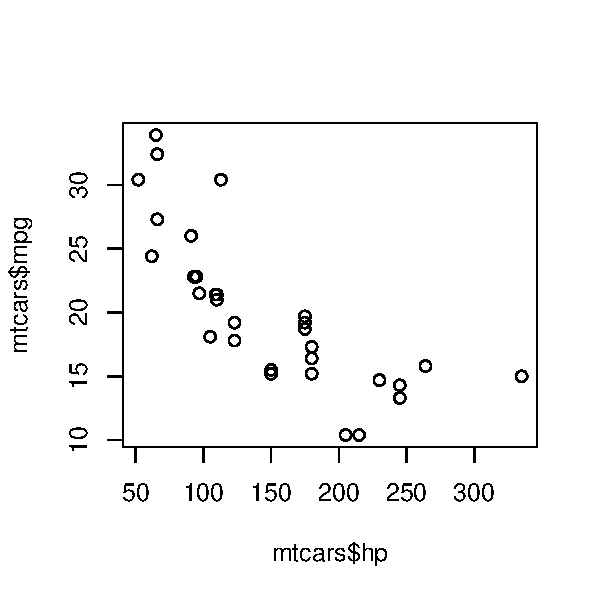
\includegraphics[width=0.45\linewidth]{Examples/Figs/mtcars-subplots-1} }
\subfloat[MPG vs Weight\label{fig:mtcars-subplots2}]{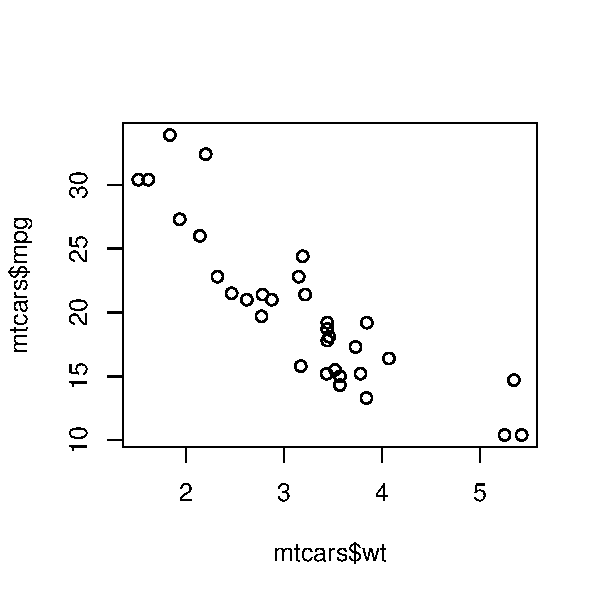
\includegraphics[width=0.45\linewidth]{Examples/Figs/mtcars-subplots-2} }

}

\caption[Plots using \texttt{mtcars} dataset]{Plots using \texttt{mtcars} dataset.}\label{fig:mtcars-subplots}
\end{figure}


\end{knitrout}




\section{Tables}
\label{sec:tables}

Tables can also be created in \R{} and inserted automatically. Check Table~\ref{tab:co2_head}.

% latex table generated in R 3.2.4 by xtable 1.8-2 package
% Sun Mar 13 14:41:42 2016
\begin{table}[htbp]
\centering
\caption[First rows of the CO2 dataset]{First rows of the CO2 dataset. Look at the list of tables to see the difference between short and long table caption.} 
\label{tab:co2_head}
\begin{tabular}{lccccc}
  \toprule
 & Plant & Type & Treatment & conc & uptake \\ 
  \midrule
1 & Qn1 & Quebec & nonchilled & 95.00 & 16.00 \\ 
  2 & Qn1 & Quebec & nonchilled & 175.00 & 30.40 \\ 
  3 & Qn1 & Quebec & nonchilled & 250.00 & 34.80 \\ 
  4 & Qn1 & Quebec & nonchilled & 350.00 & 37.20 \\ 
  5 & Qn1 & Quebec & nonchilled & 500.00 & 35.30 \\ 
  6 & Qn1 & Quebec & nonchilled & 675.00 & 39.20 \\ 
   \bottomrule
\end{tabular}
\end{table}


Something Useful I found was that you can use the \LaTeX{} package \texttt{makecell} to insert linebreaks in table headers. See the source code for Table~\ref{tab:co2_head_2}.

% latex table generated in R 3.2.3 by xtable 1.8-2 package
% Mon Mar 14 16:35:31 2016
\begin{table}[htbp]
\centering
\caption[Same table as before but with linebreaks]{Same table as before but with linebreaks.} 
\label{tab:co2_head_2}
\begin{tabular}{lcccc}
  \toprule
\thead{Plant \\ Something} & \thead{Type \\ Yes} & \thead{Treatment \\ No} & \thead{conc \\ whatever} & \thead{uptake \\ ok} \\ 
  \midrule
Qn1 & Quebec & nonchilled & 95.00 & 16.00 \\ 
  Qn1 & Quebec & nonchilled & 175.00 & 30.40 \\ 
  Qn1 & Quebec & nonchilled & 250.00 & 34.80 \\ 
  Qn1 & Quebec & nonchilled & 350.00 & 37.20 \\ 
  Qn1 & Quebec & nonchilled & 500.00 & 35.30 \\ 
  Qn1 & Quebec & nonchilled & 675.00 & 39.20 \\ 
   \bottomrule
\end{tabular}
\end{table}




% ===========================================================================================================
% Bibliography
% ===========================================================================================================

\begin{spacing}{0.9}

\bibliographystyle{apalike}
\nocite{*}
\cleardoublepage
\bibliography{References}

\end{spacing}

% ===========================================================================================================
% Appendices
% ===========================================================================================================

\begin{appendices}

\chapter{First Appendix}

In case it's needed.

\end{appendices}

\end{document}
